\section{Implementation, Integration and Test Plan}
\subsection{Overview}
\vspace{0.5cm}
This section will discuss the implementation, integration, and testing of the DREAM application. The section aims to prevent any setbacks entailing changes on the project once started its development and do multiple tasks twice. During the time that a team starts to develop a project, they have lots of ups and downs, maybe, they have had lots of bugs in their projects during the development phase and remove them easily. But as you may know, the cost of removing these bugs after publishing the application would be much more, so verification and validation play an important role in the development phase.

\subsection{Implementation Plan}
\vspace{0.5cm}

First of all, it is important to divide the project into smaller components in order to have more concrete goals that help keep the developers’ motivation high and make a straightforward development of the project. Therefore, we will divide the project into different components, starting from the ones that are responsible for the basic features and going on until the end, where we will develop the most specific ones. It is not a new method, because it has been studied during this course and it is referred to as ‘bottom-up’ strategy. This method will help to provide better integration of the project tier-by-tier and make different tests of the behavior of the application before it ends.\\
In the bottom-up approach, the implementation must start from the lower components up to the top because in this approach the implementation is gradual. In the design, there are some components that rely on other components. Thus, it's better first start implementing with the component that other components use it.\\

Two important components that we have in our application are DataVisualization and DataAnalysis because we predict based on the data that we received from DataCollection. If we don't have enough accuracy in the data that we receive from DataColletion these components wouldn't work properly. For example, if our devices were not good enough to measure accurately, or we predict or conclude based on sparse data, or if these data couldn't fulfill the requirement of our algorithms correctly.


\subsection{Integration Strategy}
\vspace{0.5cm}

To implement and test the different functionalities of the system a bottom-up approach has been used. The following diagrams describe how the process of implementation and integration testing takes place, according to a bottom-up approach. \\

\begin{enumerate}
    
\item At first the authentication is implemented and unit tested using a driver for the components that are still under implementation. It is not a complex component, but other components rely on it to provide some services: that’s why it is implemented and tested before the others. \\
\begin{figure}[H]
  \centering
  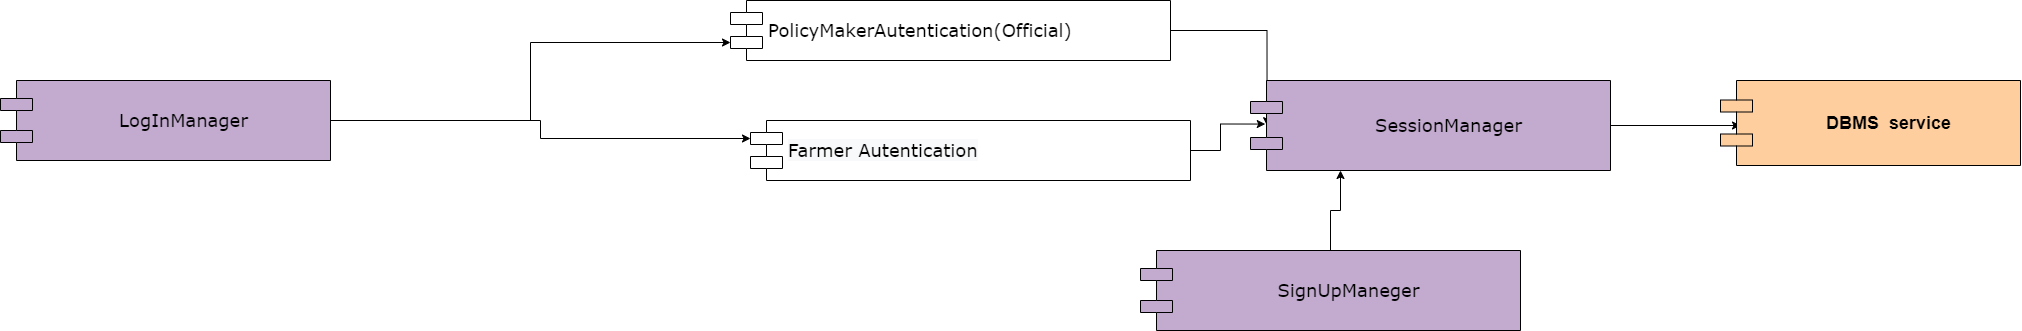
\includegraphics[width=1\textwidth,keepaspectratio]{figures/test1.png}
\end{figure}

\item Then we implement the data analyzing, because one of the most important entity of our application is analyzing the farmer progress.\\
\begin{figure}[H]
  \centering
  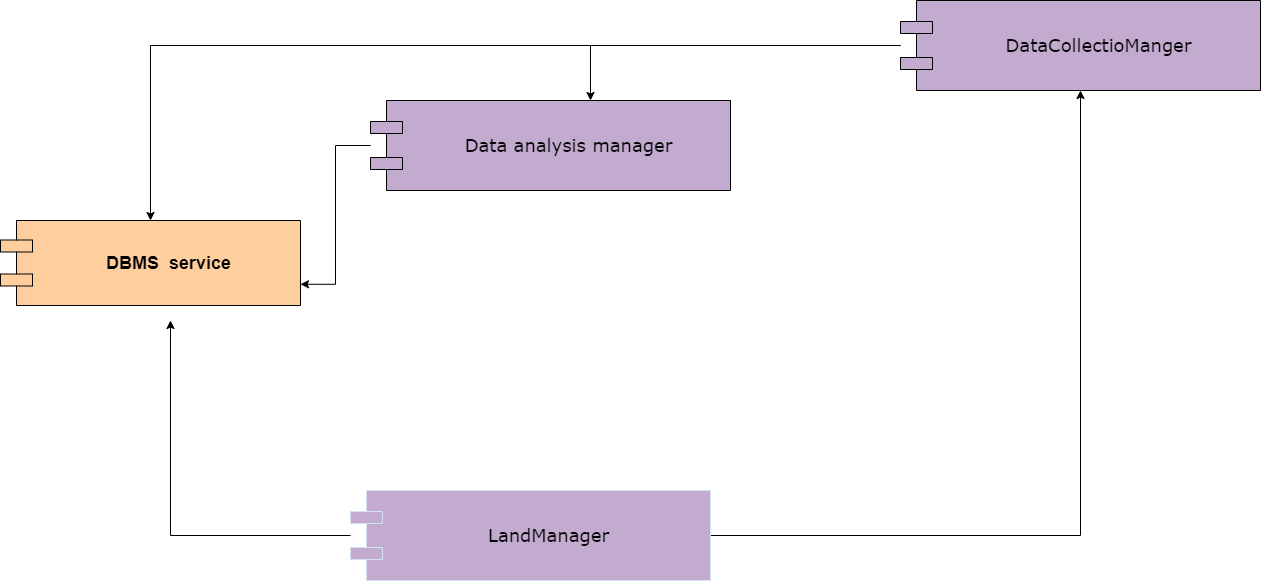
\includegraphics[width=1\textwidth,keepaspectratio]{figures/test2.png}
\end{figure}

\item another integrated components are responsible for visualize the data that analyse by analyzing component and reparation them  by data collection component.\\
\begin{figure}[H]
  \centering
  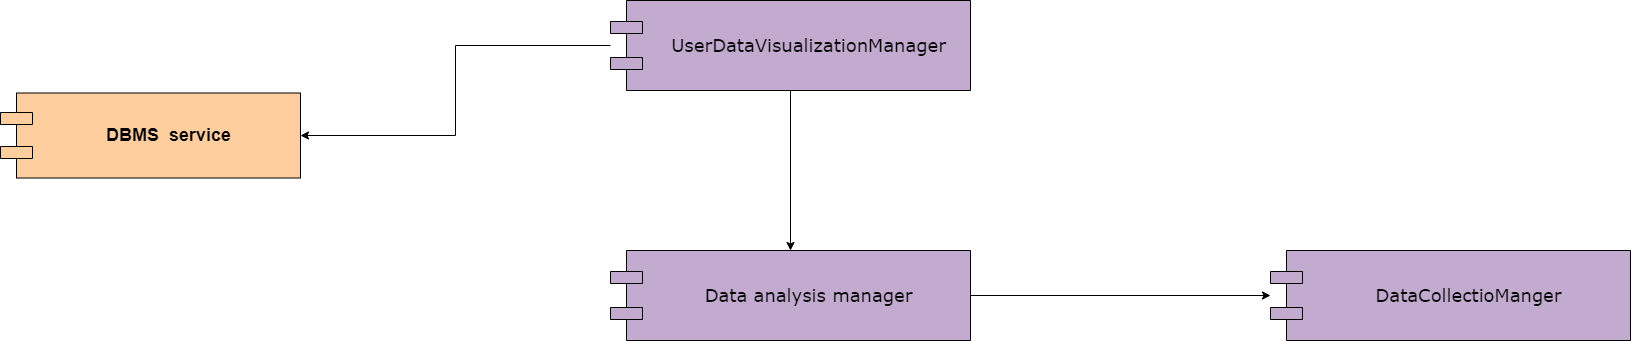
\includegraphics[width=1\textwidth,keepaspectratio]{figures/test3.png}
\end{figure}
\clearpage
\item to implement the functionality of forum for asking the question and send proper answer beside the sending  notification to related user to notice them from last changes\\
\begin{figure}[H]
  \centering
  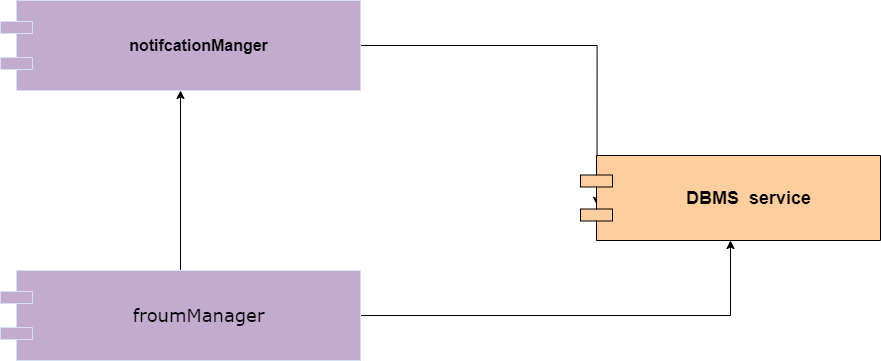
\includegraphics[width=1\textwidth,keepaspectratio]{figures/test4 (1).png}
\end{figure}

\end{enumerate}

\clearpage